\chapter{Project Organization}
\label{cha:projectorganization}


This chapter will cover how we organized the entire project. We will uncover the the project timeline in the first section. How roles are distributed among the members will be mentioned in second section and we will talk about tools used in the third section
\section{Timeline}
\begin{figure}[!ht]
	\centering
	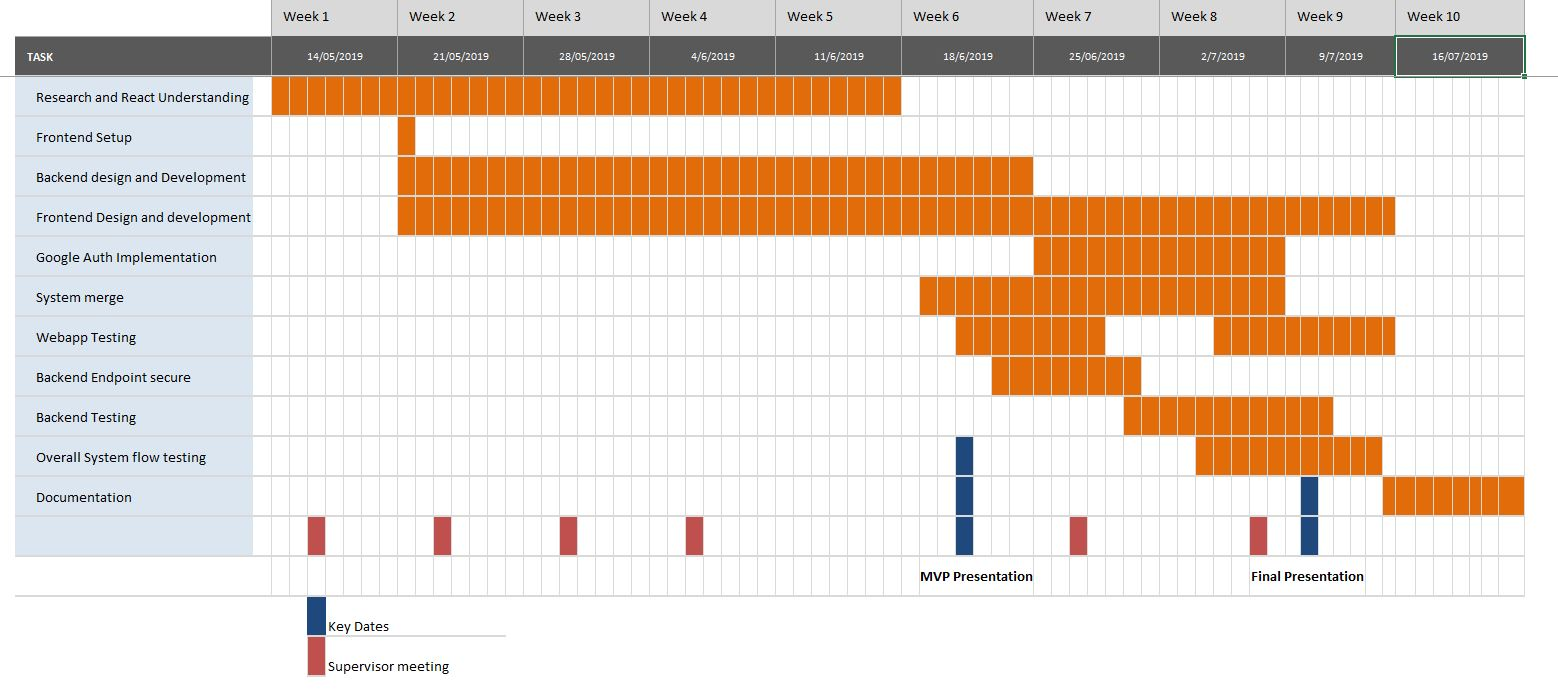
\includegraphics[width=1\textwidth]{images/Timeline.jpg}\\
	\caption{Project Timeline}
	\label{fig:Project Timeline}
\end{figure}

\section{Work Distribution}
\begin{table}[!ht]
\begin{center}
\begin{tabular}{ |l|l|l| } 
 \hline
\textbf{Task} & \textbf{Team Member} \\
 \hline
Customer & Alon \\
 \hline
Company & Kiran  \\
 \hline
 Postman & Anubhav \\
 \hline
 Integration, Routing and Common Web pages & Pradyumna \\
 \hline
 Backend & Haseeb Asif \\
 \hline
  Documentation & All Members \\
 \hline
\end{tabular}
\end{center}
    \caption{ Task Distribution }
\end{table}
To fulfill the requirement of the project in the given 10 weeks time frame, we divided the task as shown in \textbf{table 4.1}. Member who took charge of each user space design worked from the same basic design and were synchronized with each other to maintain the consistency. Github was used by all members fro source control purpose. Member responsible for each user space had the responsibility to develop the functionality of those user too. Member who was working on customer view was responsible for all customer functionality and so on for other team members. Integration, routing and common web page development task handler was responsible for login/register page, overall page routing, system integration with backend. Member with backend task was responsible for overall database design and implementation according to the need system requirement. Documentation is done by all member input. 
The table shows the major responsible person for the given task, however each member has provided input on other's jobs too. Project was collective task using input, knowledge and expertise of each and every member of the group.
\section{Tools and Infrastructure}

\begin{itemize}
\item Github - Source control (iosl-dc3, iosl-backend)
\item Trello -Task mgmt (https://trello.com/b/RXwlgcJI/iosl-dc3)
\item Slack - Communication (https://iosltu2019.slack.com)
\item Overleaf- Documentation Collaboration (https://overleaf.com)
\item VS Code - Code editor
\item Azure for Postgres SQL - Database
\end{itemize}